\documentclass[journal]{journal}
\usepackage{subcaption}
\usepackage{graphicx}
\usepackage{url}
\usepackage{color}
\usepackage{multirow}
\usepackage{makecell}
\usepackage{mathptmx}
\usepackage{amsmath}
%define some own functions
\newcommand{\tabincell}[2]{\begin{tabular}{@{}#1@{}}#2\end{tabular}} 
\def\D{\mathrm{d}}
% correct bad hyphenation here
\hyphenation{op-tical net-works semi-conduc-tor}
\pagestyle{empty}
\begin{document}

\title{Real-Time Recognition of Dynamic Hand Postures on a Neuromorphic System}
\author{
Qian~Liu, 
and~Steve~Furber,~\IEEEmembership{Fellow,~IEEE}
\thanks{
The authors are with the School of Computer Science, University of Manchester, Manchester M13 9PL, U.K. 
(e-mail:qian.liu-3@manchester.ac.uk; steve.furber@manchester.ac.uk).}
}% <-this % stops a space
%\thanks{Manuscript received April 19, 2005; revised January 11, 2007.}}

\maketitle
\thispagestyle{empty}

\begin{abstract}
%To explore the visual processing of the brain, this paper proposes a real-time recognition system for dynamic hand postures on a neuromorphic platform.
%The hardware system includes a front-end of a Dynamic Video Sensor~(DVS) silicon retina and a real-time Spiking Neural Network~(SNN) simulator, SpiNNaker, as the back-end.
%The neural network model is tested both on Matlab and SpiNNaker to validate the transformation from rate-based linear perceptrons to spiking Leaky Integrate-and-Fire (LIF) neurons.
%Live recognition with real-time retina input is also carried out to test both the hardware platform and the model.
%Moreover, different network sizes are configured to evaluate the cost and performance trade-off.
%Motivation
%To explore how brain may recognise object in its general, accurate and energy-efficient manner, this paper proposes a neuromorphic hardware system which includes a Dynamic Video Sensor~(DVS) silicon retina connected to SpiNNaker, a real-time Spiking Neural Network~(SNN) simulator.
%%Problem
%Building a recognition system based on the bespoke hardware for dynamic hand postures is a first step to study the visual pathway of the brain.
%%Methods
%Inspired by the approaches of the primary visual cortex, convolutional neural networks are modelled using both linear perceptrons and spiking Leaky Integrate-and-Fire (LIF) neurons.
%%Results
%The larger network of 74,210 neurons and 15,216,512 synapses runs smoothly in real-time on SpiNNaker taking 290 cores of a 48-node board.
%The smaller network using 1/10 of the resources is able to recognise the postures in real-time with an accuracy about 86.4\% in average, which is 
%only 6.6\% lower than the former.
%%Concolusion
%The recognition rate of the smaller network is adequate for a hand posture recognition system with a better cost and performance trade-off.

To explore how the brain may recognise objects in its general,accurate and energy-efficient manner, this paper proposes the use of a neuromorphic hardware system formed from a Dynamic Video Sensor~(DVS)
silicon retina in concert with the SpiNNaker real-time Spiking Neural
Network~(SNN) simulator.
As a first step in the exploration on this platform a recognition system for dynamic hand postures is developed, enabling the study of the methods used in the visual pathways of the brain.
Inspired by the behaviours of the primary visual cortex, Convolutional Neural Networks (CNNs) are modelled using both linear perceptrons and spiking Leaky Integrate-and-Fire (LIF) neurons.

In this study's largest configuration using these approaches, a network of 74,210 neurons and 15,216,512 synapses is created and operated in real-time using 290 SpiNNaker processor cores in parallel and with 93.0\% accuracy.
A smaller network using only 1/10th of the resources is also created,
again operating in real-time, and it is able to recognise the postures
with an accuracy of around 86.4\% - only 6.6\% lower than the much larger system.
The recognition rate of the smaller network developed on this neuromorphic system is sufficient for a successful hand posture recognition system, and demonstrates a much improved cost to performance trade-off in its approach.

 
\end{abstract}

\begin{IEEEkeywords}
spiking neural network (SNN), convolutional neural network (CNN), posture recognition, neuromorphic system.
\end{IEEEkeywords}

\section{Introduction}
\IEEEPARstart{P}{atterns} or objects in two-dimensional images can be described with four properties~\cite{wysoski2008fast}: position, geometry (i.e. size, area and shape), colour/texture, and trajectory. 
Appearance-based methods are the most direct approach to performing pattern recognition where the test image is compared with a set of templates to find the best match for an individual or combination of properties. 
%In terms of classification algorithms, distance measure methods (nearest neighbour, k-means clustering), support vector machine (SVM), multi-layer perceptron (MLP) neural networks and statistical methods, e.g. Gaussian mixture model (GMM) have been applied successfully in visual recognition. 
However, the 2D projection of an object changes under different conditions including illumination, viewing angles, relative positions and distance, making it virtually impossible to represent all appearances of an object. 
To improve reliability, robustness and classification efficiency, approaches such as edge matching~\cite{canny1986computational}, divide-and-conquer~\cite{toygar2004multiple}, gradient matching~\cite{wei2006robust} and feature based methods~\cite{lowe2004distinctive, bay2008speeded} are used.
%Moreover, feature based methods are used to improve reliability, robustness and classification efficiency. 
%Among various feature extraction methods, the scale-invariant feature transform (SIFT)~\cite{lowe2004distinctive} and the sped-up robust features (SURF)~\cite{bay2008speeded} methods are well-accepted recently in the field. 
Finding a proper feature for a specific object still remains an open question and there is no process as general, accurate, or energy-efficient as that provided by the brain.
It is not a new idea to turn to nature for inspiration. 
%Turning to biology for answers is always the way to explore the field of visual pattern recognition. 
Riesenhuber et al.~\cite{riesenhuber1999hierarchical}, for instance, presented a biologically-inspired model based on the organisation of the visual cortex which has the ability to represent relative position- and scale-invariant features.
Integrating a rich set of visual features became possible using a feed-forward hierarchical pathway. 

To explore how brain may recognise objects, we have employed a biologically-inspired DVS silicon retina~\cite{lenero20113}, a good example of low-cost visual processing due to its event-driven and redundancy-reducing style of computation;
and a SpiNNaker system~\cite{furber2014spinnaker}, which is a massive parallel computing platform aimed at real-time simulation of SNNs. 
%SpiNNaker, as the back-end of the system, provides a flexible, event-driven mechanism for real-time simulation of SNNs, and is where the posture recogniser locates.
With this neuromorphic hardware system we have the ability to explore visual processing by mimicking the functions of various regions along the visual pathway. 
Building a real-time recognition system for dynamic hand postures is a first step of exploring visual processing in a biological fashion and is also a validation of the neuromorphic platform.
To match the image properties detailed earlier, the position, shape, size and trajectory of the hand postures can be detected from the retina output.
To keep the task simple at first, the postures are of similar size and the goal is to recognise the shape of a hand with moving positions.
Tracking the postures with a short memory will form part of the future work.

Dynamic recognition takes advantage of the intrinsic temporal processing of SNNs which are receiving considerable attention for  undertaking vision processing.
Pattern information can be encoded in the delays between the pre- and post-synaptic spikes since the spiking neurons are capable of computing radial basis functions (RBFs)~\cite{hopfield1995pattern}.
Spatio-temporal information can also be stored in the exact firing time rather than relative delays~\cite{natschlager1998spatial}.
%Maass~\cite{maass1997networks} has proved mathematically that:
%1) networks of spiking neurons are computationally more powerful than the first and second generation of neural network models;
%2) a concrete biologically relevant function can be computed by a single spiking neuron, replacing  hundreds of hidden units in a sigmoidal neural net;
%3) any function that can be computed by a small sigmoidal neural net can also be computed by a small network of spiking neurons.
Numerous applications using SNN-based vision processing have been successfully carried out in the past. 
A dual-layer SNN has been trained using Spike Time Dependent Plasticity (STDP) and employed for character recognition~\cite{gupta2007character}. 
Lee et al.~\cite{6467270} have implemented direction selective filters in real time using spiking neurons, considered as a convolution layer in the model of a so called CNN~\cite{camunas2012event}. 
Different features, such as Gabor filter features (scale, orientation and frequency) and shape can be modelled as layers of feature maps. 
The similar behaviours have been found in the primary visual cortex (V1) in the visual pathway~\cite{rehn2007network} as the foundation for higher level visual process e.g. object recognition.
%Rank order coding, as an alternative to conventional rate-based coding, treats the first spike as the most important and has been successfully applied to an orientation detection training process~\cite{delorme2001networks}. 
%Nengo~\cite{eliasmith2011nengo} is a graphical and scripting based software package for simulating large-scale neural systems and has been used to build the world's largest functional brain model, Spaun~\cite{eliasmith2012large}. 
%An FPGA implementation of a Nengo model for digit recognition has been reported~\cite{naylor2013managing}. 
Deep Belief Networks (DBNs), the 4th generation of artificial neural network, have shown great success in solving classification problems. 
Recent study~\cite{o2013real} in this area has mapped an offline-trained DBN onto an efficient event-driven spiking neural network for digit recognition tasks with resounding success.

Section~\ref{sec:np} of this paper presents the details of the hardware of the proposed neuromorphic system, including the silicon retina and the SpiNNaker platform.
The neural network models are defined and tested on Matlab, and the model structures and experimental results stated in Section~\ref{sec:cnn}.
In Section~\ref{sec:rrs}, the rate-based models are converted into spiking neurons, and real-time live recognition and recorded data experiments are carried out.
The contribution of this work is summarised and the future directions are provided in Section~\ref{sec:cfw}.
% which is a massive parallel computing platform aimed at real-time simulation of spiking neural networks (SNNs). 

\section{The Neuromorphic Platform}
\label{sec:np}
The outline of the platform is illustrated in Figure~\ref{fig:SysOverViewa}, where the hardware system is configured, controlled and monitored by the PC.
%Figure~\ref{fig:SysOverViewb} shows the combined hand posture recognition system; 
The jAER~\cite{delbruck2008frame} event-based processing software on the PC configures the retina and displays the output spikes through a USB link.
The host communicates to the SpiNNaker board via Ethernet to set up its runtime parameters and to download the neural network model off-line.
It visualises~\cite{6252490} the spiking activity of the network in real-time.
The photograph of the hardware platform, Figure~\ref{fig:SysOverViewb}, shows that the silicon retina connects to the SpiNNaker 48-node system via a Spartan-6 FPGA board~\cite{galluppi2012real}.
%, which was also applied to a sound localisation system.


\begin{figure}
\centering
	\begin{subfigure}[t]{0.4\textwidth}
		\includegraphics[width=\textwidth]{pics/outline.pdf}
	    \caption{Outline of the platform.}
	    \label{fig:SysOverViewa}
	\end{subfigure}
	\\
	\begin{subfigure}[t]{0.48\textwidth}
		\includegraphics[width=\textwidth]{pics/outline2.pdf}	    \caption{Picture of the hardware platform. From left to right: a silicon retina, a FPGA board, and a 48-node SpiNNaker system.}
	    \label{fig:SysOverViewb}
	\end{subfigure}	

\caption{System overview of the dynamic hand posture recognition platform. 
%The silicon retina connects to the SpiNNaker system through an FPGA board. 
%Spikes from the retina are streamed to the SpiNNaker system through this Spartan-6 FPGA board.
%The jAER software configures the retina and displays its outgoing spikes through the USB connection.
%The host sets up the runtime parameters off-line and downloads the network model to the SpiNNaker system.
}
\label{fig:SysOverView}
\end{figure}

\subsection{Silicon Retina}
The visual input is captured by a DVS silicon retina, which is quite different from conventional video cameras.
Each pixel generates spikes when its change in brightness reaches a defined threshold.
Thus, instead of buffering video into frames, the activity of pixels is sent out and processed continuously with time.
The communication bandwidth is therefore optimised by sending activity only, which is encoded as pixel events using Address-Event Representation (AER~\cite{lazzaro1995multi}) protocol.
The level of activity depends on the contrast change; pixels generate spikes faster and more frequently when they are subject to more active change.
The sensor is capable of capturing very fast moving objects (e.g., up to 10 K rotations per second), which is equivalent to 100 K conventional frames per second~\cite{lenero20113}.

\subsection{SpiNNaker System}
The SpiNNaker project's architecture mimics the human brain's biological structure and functionality. 
This offers the possibility of utilizing massive parallelism and redundancy, as the brain, to provide resilience in an environment of unreliability and failure of individual components.

In the human brain, communication between its computing elements, or neurons, is achieved by the transmission of electrical `spikes' along connecting axons. 
The biological processing of the neuron can be modelled by a digital processor and the axon connectivity can be represented by messages, or information packets, transmitted between a large number of processors which emulate the parallel operation of the billions of neurons comprising the brain.

The engineering of the SpiNNaker concept is illustrated in Figure~\ref{fig:sysdia} where the hierarchy of components can be identified. 
Each element of the toroidal interconnection mesh is a multi-core processor known as the `SpiNNaker Chip' comprising 18 processing cores. 
Each core is a complete processing sub-system with local memory.
It is connected to its local peers via a Network-on-Chip (NoC) which provides high bandwidth on-chip communication and to other SpiNNaker chips via links between them. 
In this way massive parallelism extending to thousands or millions of processors is possible.

\begin{figure}
\centering
	\includegraphics[width=0.42\textwidth]{pics/mesh_ctiff.jpg}
	\caption{SpiNNaker system diagram.
	Each element represents one chip with local memory.
	Every chip connects to its neighbours through the six bi-directional on-board links. }
	\label{fig:sysdia}
\end{figure}

%The knowledge content and learning ability of the brain is generally thought to be embodied in its evolvable interconnection pattern.
%This structure routes a spike generated by one neuron to others which are interconnected with it via axons and these interconnections are modified and extended as a result of learning processes.
%
%In SpiNNaker a packet router within each multi-core processor controls the neural interconnection. 
%Each transmitted packet represents a spike and simply identifies its source neuron.
%This is used by routers to identify whether a packet should be routed to a processor core, or should be routed on to one of the six adjacent chips connected to it as part of the overall SpiNNaker network.

The `103 machine' is the name given to the 48-node board which we use for the hand posture recognition system, see Figure~\ref{fig:SysOverViewb}.
It has 864 ARM processor cores, typically deployed as 768 application, 48 monitor and 48 spare cores. 
%The `103 machine' requires a 12V 6A supply. 
%The control interface is via two 100Mbps Ethernet connections, one for the board management processor and the second for the SpiNNaker array. 
%There are options to use the nine on-board 3.0~Gbps high-speed serial interfaces (using SATA cables, but not necessarily the SATA protocol) for I/O; 
%this will require suitable configuration of the on-board FPGAs that provide the high-speed serial interface support. 
The boards can be connected together to form larger systems using high-speed serial interfaces. 

%\begin{figure}
%\centering
%	\includegraphics[width=0.42\textwidth]{pics/SpiNN5.pdf}
%	\caption{`103 Machine' PCB}
%	\label{fig:48node}
%\end{figure}

\subsection{Interfacing AER Sensors}
Spikes from the silicon retina are injected directly into SpiNNaker via a SPARTAN-6 FPGA board that translates them into a SpiNNaker compatible AER format~\cite{appnote8}. 

From a neural modelling point of view, interfacing the silicon retina is performed using pyNN~\cite{davison2008pynn}. 
The retina is configured as a spike source population that resides on a virtual SpiNNaker chip, to which an AER sensor's spikes are directed, thus abstracting away the hardware details from the user\cite{galluppi2012real}.
Besides the retina, we have successfully connected an AER based silicon cochlea~\cite{5537164} to SpiNNaker for a sound localisation task~\cite{6706931}.

\section{Convolutional Neural Networks}
\label{sec:cnn}
The convolutional network is well-known as an example of a biologically-inspired model. 
Figure~\ref{fig:conv} shows a typical convolutional connection between two layers of neurons. 
The repeated convolutional kernels are overlapped in the receptive fields of the input neurons. 
\begin{figure}
\centering
	\includegraphics[width=0.42\textwidth]{pics/conv.pdf}
	\caption{Each individual neuron in the convolution layer (right matrix) connects to its receptive field using the same kernel. The value of the kernel is represented by the synaptic weights between the connected neurons.}
	\label{fig:conv}
\end{figure}

\subsection{Model Description}
\label{sec:mds}
There are two CNNs proposed to accomplish the dynamic hand posture recognition task.
A straight forward method of template matching is employed at first, followed by a network of multi-layer perceptrons (MLP) trained to improve the recognition performance.


\begin{figure}
\centering
	\includegraphics[width=0.48\textwidth]{pics/model1.pdf}
	\caption{Model 1. 
	The retina input is convolved with Gabor filters in the second layer, and then shrinks the sizes in the pooling layer.
	The templates are considered as convolution kernels in the last layer.
	The WTA circuit can be used as an option to show the template matching result more clearly.
	}
	\label{fig:model1}
\end{figure}
%\subsubsection{Model 1. Template Matching}

Model 1: Template Matching. Shown in Figure~\ref{fig:model1} the first layer is the retina input, followed by the convolutional layer, where the kernels are Gabor filters responding to edges of four orientations.
The third layer is the pooling layer where the size of the populations shrinks. 
This down-sampling enables robust classification due to its tolerance to variations in the precise shape of the input. 
The fourth layer is another convolution layer where the output from the pooling layer is convolved with the templates.
The optional layer of Winner-Take-All (WTA) neurons enables a clearer classification result due to the inhibition between the neurons.
In the Matlab simulation, the retina input spikes are buffered into 30~ms frames, and the neurons are simple linear perceptrons.
The templates are chosen by sampling the output of the pooling layer when given some reference stimulus, see Figure~\ref{fig:template}.

\begin{figure}
\centering
	\includegraphics[width=0.48\textwidth]{pics/gesture.pdf}
	\caption{Templates of the five postures: `Fist',`Index Finger', `Victory Sign', `Full Hand' and `Thumb up'.}
	\label{fig:template}
\end{figure}

The Gabor filter is well-known as a linear filter for edge detection in image processing. 
A Gabor filter is a 2D convolution of a Gaussian kernel function and a sinusoidal plane wave; see Equation~\ref{equ:gabor}. 
\begin{equation}
\begin{array}{l}
\mathrm{Real Parts} = \exp \left(\frac{-x^{'2}+y^{'2}}{2\sigma ^{2}}\right)\cos \left(2\pi\frac{{x}'}{\lambda }\right)
\\
\\
\mathrm{Imaginary Parts} = \exp \left(\frac{-x^{'2}+y^{'2}}{2\sigma ^{2}}\right)\sin \left(2\pi\frac{{x}'}{\lambda }\right)
\\
\\
\mathrm{where:}
\\
\\
{x}'=x\cos (\theta ) + y\sin (\theta)
\\
\\
{y}'=-x\sin (\theta ) + y\cos (\theta)
\end{array}
\label{equ:gabor}
\end{equation}
$\theta$ represents the orientation of the filter, $\lambda$ is the wavelength of the sine wave, and $\sigma$ is the standard deviation of the Gaussian envelope. 
The frequency and orientation features are similar to the responses of V1 neurons in the human visual system. 
Only the real parts of the Gabor filters (see Figure~\ref{fig:gabor}) are used as the convolutional kernels to configure the weights between the input layer and the Gabor filter layer.

\begin{figure}
\centering
	\includegraphics[width=0.48\textwidth]{pics/gabor.pdf}
	\caption{Real parts of the Gabor filters orienting four directions.}
	\label{fig:gabor}
\end{figure}

%The templates (see Figure~\ref{fig:template}) are manually selected from the output of the pooling layer in the framed Matlab simulation. 
The output score of a convolution is determined by the matching degree between the input and the kernel.
Regarding the template matching layer, each neuron in a population responds to how closely its receptive field matches the specific template.
The position of moving gesture is also naturally encoded in the address of template matching neuron.
Thus, there are five populations of template matching neurons, one for each hand posture listed.

%\subsubsection{Model 2. Trained MLP}
Model 2: Trained MLP. 
Inspired by the research of Lecun~\cite{lecun1998gradient}, we designed a combined network model with MLP and CNN (Figure~\ref{fig:model2}). 
The first three layers are exactly the same as the previous model.
The training images for the 3-layered MLP are of same size and the posture is centred in the images.
Therefore, a tracking layer plays an important role to find the most active region and forward the centred image to the next layer.

\begin{figure}
\centering
	\includegraphics[width=0.52\textwidth]{pics/model2.pdf}
	\caption{Model 2. 
	The retina input convolves with Gabor filters in the second layer, and then shrinks the sizes in the pooling layer.
	The following tracking layer finds the most active area of some fixed size, moves the posture to the centre and pushes the image to the trained MLP.
	The winner-take-all (WTA) layer can be used as an option to show the template matching result more clearly.}
	\label{fig:model2}
\end{figure}

%Since the size of the input image of the MLP training is fixed and the position is centered, tracking plays a very important role to spot the valid region. 
%Tracking is naturally embedded in the pooling layer of the convolutional network, for the active neurons directly point out the lively receptive field. 

\subsection{Experimental Set-up}
\label{sec:tat}
In order to evaluate the cost and performance trade-offs in optimizing the number of neural components, both the convolutional models described above are tested at different scales. 
Five videos of every posture are captured from the silicon retina in AER format, all of similar size and moving clock-wise in front of the retina. 
The videos are cut into frames (30~ms per frame) and presented to the convolutional networks. 
The configurations of the networks are listed in Table~\ref{tbl:nns}.
The integration layer is not necessary in a convolutional network, but is used here to decrease the number of synaptic connections.

\begin{table}
\caption{Sizes of the convolutional neural networks.}
	\begin{subtable}{0.5\textwidth}
		
		\centering
		\caption{Model 1: Template matching}
		\begin{tabular}{p{0.13\textwidth}|p{0.15\textwidth}<{\centering}|p{0.13\textwidth}<{\centering}|p{0.13\textwidth}<{\centering}|p{0.13\textwidth}<{\centering}}
		%Line 1
		\Xhline{1.2pt}
		    & \multicolumn{2}{c|}{\tabincell{c}{\textbf{Full Resolution } \\\textbf{128 $\times$ 128}}}  
		    & \multicolumn{2}{c}{\tabincell{c}{\textbf{Sub-sampled Resolution} \\\textbf{32 $\times$ 32}}}
		    \\ \cline{2-5}
		%Line 2
			& \tabincell{c}{Population \\ Size}
			& \tabincell{c}{Connections \\ per Neuron}
			& \tabincell{c}{Population \\ Size}
			& \tabincell{c}{Connections \\ per Neuron}
			\\ \Xhline{1.2pt}
		%Line 3
		\tabincell{l}{\textbf{Retinal} \\\textbf{Input}}
			& 128 $\times$ 128	& 1	& 32 $\times$ 32	& 4 $\times$ 4
			\\ \hline
		%Line 4
		\tabincell{l}{\textbf{Gabor} \\\textbf{Filter}}
			& 112$\times$112$\times$4	& 17 $\times$ 17	& 28$\times$28$\times$4	& 5 $\times$ 5
			\\ \hline
		%Line 5
		\tabincell{l}{\textbf{Pooling} \\\textbf{Layer}}
			& 36$\times$36$\times$4	& 5 $\times$ 5	& null	& null
			\\ \hline
		%Line 6
		\tabincell{l}{\textcolor[rgb]{0.55,0.55,0.55}{\textbf{Integration}} \\ \textcolor[rgb]{0.55,0.55,0.55}{\textbf{Layer}}}
			& 36 $\times$ 36	& 4	& 28 $\times$ 28	& 4
			\\ \hline
		%Line 7
		\tabincell{l}{\textbf{Template} \\\textbf{Matching}}
			& 16$\times$16$\times$5	& 21 $\times$ 21	& 14$\times$14$\times$5	& 15 $\times$ 15
			\\ \Xhline{1.2 pt}
		%Line 8
		\textbf{Total}
			& $74,320$	& $15,216,512$	& $5,925$	& $318,420$
			\\ \Xhline{1.2 pt}
		\end{tabular}
		\label{tbl:m1}
	\end{subtable}
	\par\bigskip
	\begin{subtable}{0.5\textwidth}
		
		\centering
		\caption{Model 2: Trained MLP}
		\begin{tabular}{p{0.13\textwidth}|p{0.15\textwidth}<{\centering}|p{0.13\textwidth}<{\centering}|p{0.13\textwidth}<{\centering}|p{0.13\textwidth}<{\centering}}
		%Line 1
		\Xhline{1.2pt}
		    & \multicolumn{2}{c|}{\tabincell{c}{\textbf{Full Resolution} \\\textbf{128 $\times$ 128}}}  
		    & \multicolumn{2}{c}{\tabincell{c}{\textbf{Sub-sampled Resolution} \\\textbf{32 $\times$ 32}}}
		    \\ \cline{2-5}
		%Line 2
			& \tabincell{c}{Population \\ Size}
			& \tabincell{c}{Connections \\ per Neuron}
			& \tabincell{c}{Population \\ Size}
			& \tabincell{c}{Connections \\ per Neuron}
			\\ \Xhline{1.2pt}
		%Line 3
		\tabincell{l}{\textbf{Tracked} \\\textbf{Input}}
			& 21 $\times$ 21	& null	& 15 $\times$ 15	& null
			\\ \hline
		%Line 4
		\tabincell{l}{\textbf{Hidden} \\\textbf{Layer}}
			& 10	& 21$\times$21$\times$10	& 10	& 15$\times$15$\times$10
			\\ \hline
		%Line 5
		\tabincell{l}{\textbf{Recognition} \\\textbf{Layer}}
			& 5	& 5$\times$10	& 5	& 5$\times$10
			\\ \Xhline{1.2pt}
		%Line 6
		\textbf{Total}
			& $456$	& $4,460$	& $240$	& $2,300$
			\\ \Xhline{1.2 pt}
		\end{tabular}
		\label{tbl:m2}
	\end{subtable}
	\label{tbl:nns}
\end{table}

\subsection{Experimental Results}
\label{sec:exp}

\begin{figure}
\centering
	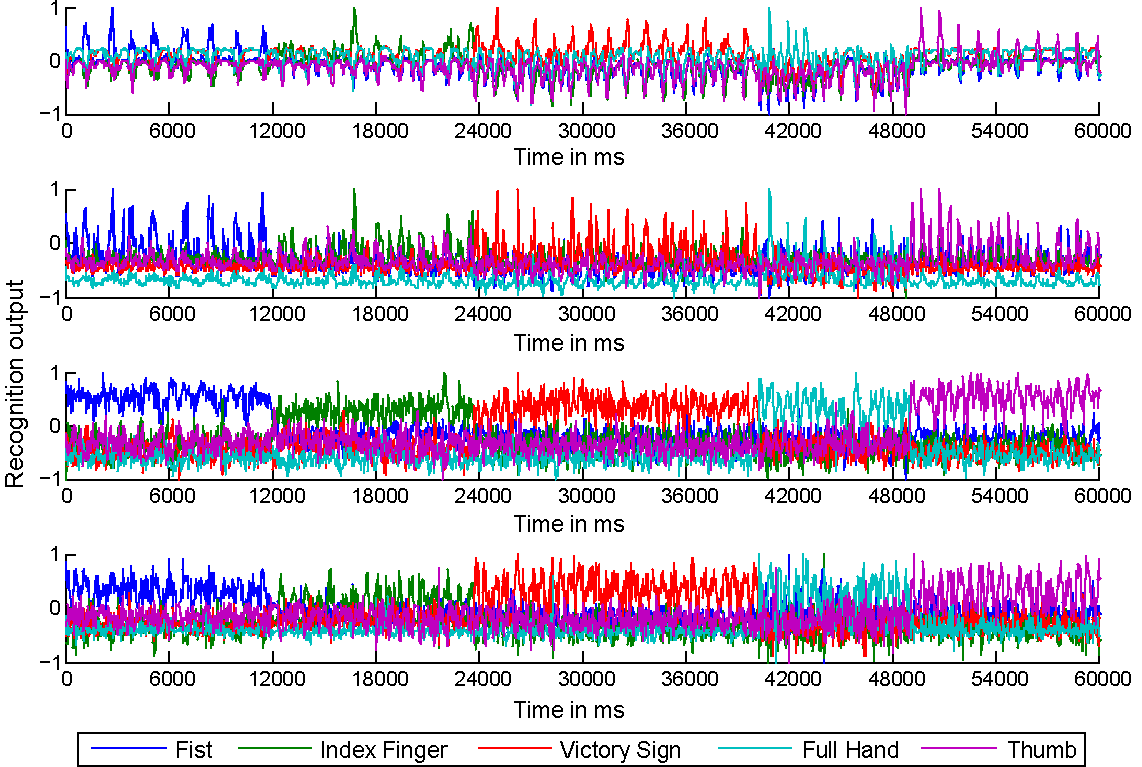
\includegraphics[width=0.48\textwidth]{pics/rateMatlab.pdf}
	\caption{Neural responses with time of four experiments to the same recorded moving postures.
	The recognition output is normalised to \mbox{[-1, 1]}.
	Every point represents the highest response in a specific population (different colour) for a 30~ms frame.
	The 1st plot refers to Model 1 with the full input resolution, and the 2nd plot Model 1 with the sub-sampled input resolution; and the 3rd and fourth plots both refer to Model 2, and with high and low input resolution respectively. 
	}
	\label{fig:matlabrec}
\end{figure}




In Figure~\ref{fig:matlabrec} the first two plots refer to Model 1, using template matching. Each colour represents one of the recognition populations. 
Each point in the plot is the highest neuronal response in the recognition population during the time of one frame (30~ms). 
The neuronal response, `the spiking rate', is normalised to [-1, 1]. 
It can be seen that the higher resolution input makes the boundaries between the classes clearer. 
On the other hand, recognition only happens when the test image and template are similar enough. 
The templates are only selected from the frames where the gestures are moving towards the right, and the gestures are moving clockwise in the videos, thus, all the peaks in plot 1 correspond with moments when the gesture moves towards right.  
It is notable that the higher resolution causes the recogniser to be more sensitive to the differences between the test data and the template, while the smaller neural network can recognize more generalized patterns. 
Therefore, a threshold is required to differentiate between data that is close enough and that which is not. 
Since the gestures are moving in four different directions during the clockwise movement, a rejection rate (i.e. none of the template is matched) of 75\% is to be expected. 

The latter two plots of Figure~\ref{fig:matlabrec} refer to Model 2. 
The three-layer MLP network significantly improves the recognition rate and can generalise the pattern. 
There is no rejection rate for Model 2, since the MLP is trained with all the moving directions of the postures.

Detailed results are listed in Table~\ref{tbl:rsl}. 
The correct recognition rate is calculated from the non-rejected frames.
The lower resolution of the 32$\times$32 retina input is adequate (85.83\%) for this gesture recognition task. 
The smaller network uses only 1/10th the number of neurons and 1/50th the number of synaptic connections compared with the full resolution network, while the recognition rate drops only around by 9.0\% with Model 1 and 17.2\% with Model 2.

\begin{table}
\centering
\caption{Recognition results using linear perceptrons in \%}
	\begin{tabular}{p{0.075\textwidth}|p{0.05\textwidth}<{\centering}|p{0.055\textwidth}<{\centering}|p{0.055\textwidth}<{\centering}|p{0.055\textwidth}<{\centering}|p{0.055\textwidth}<{\centering}}
		%Line 1
		\Xhline{1.2pt}
		    \multicolumn{2}{c|}{}	& \multicolumn{2}{c|}{\textbf{Model 1}}  
		    & \multicolumn{2}{c}{\textbf{Model 2}}
		    \\ \cline{3-6}
		%Line 2
		\multicolumn{2}{c|}{}	& \tabincell{c}{High \\ Resolution}
			& \tabincell{c}{Low \\ Resolution}
			& \tabincell{c}{High \\ Resolution}
			& \tabincell{c}{Low \\ Resolution}
			\\ \Xhline{1.2pt}
		%Line 3-4	
		\multirow{2}{*}{\tabincell{l}{\textbf{Fist}\\ (399 Frames)}}
			& Correct & 99.11	& 99.23	& 96.24	& 84.21
			\\ \cline{2-6}
			& Reject  & 71.93 & 67.42 	& Null	& Null
			\\ \hline
		%Line 5-6
		\multirow{2}{*}{\tabincell{l}{\textbf{Index Finger} \\ (392 Frames)}}
			& Correct & 92.98	& 80.00	& 94.39	& 71.69
			\\ \cline{2-6}
			& Reject & 70.92	& 75.77 	& Null	& Null
			\\ \hline
		%Line 7-8
		\multirow{2}{*}{\tabincell{l}{\textbf{Victory Sign} \\ (551 Frames)}}
			& Correct & 96.56	& 93.07	& 95.64	& 87.66
			\\ \cline{2-6}
			& Reject & 73.68	& 81.67 	& Null	& Null
			\\ \hline
		%Line 9-10
		\multirow{2}{*}{\tabincell{l}{\textbf{Full Hand} \\ (293 Frames)}}
			& Correct & 95.65	& 72.41	& 93.52	& 72.01
			\\ \cline{2-6}
			& Reject & 92.15	& 90.10 	& Null	& Null
			\\ \hline
		%Line 10-11
		\multirow{2}{*}{\tabincell{l}{\textbf{Thumb up} \\ (391 Frames)}}
			& Correct & 89.61	& 84.44	& 96.68	& 74.68
			\\ \cline{2-6}
			& Reject & 80.31	& 76.98 	& Null	& Null
			\\ \hline\hline
		\multirow{2}{*}{\tabincell{l}{\textbf{Average}}}
			& Correct & 94.78	& 85.83	& 95.29	& 78.05
			\\ \cline{2-6}
			& Reject & 77.80	& 78.39 	& Null	& Null
			\\ \hline
	\end{tabular}
	\label{tbl:rsl}
\end{table}


\section{Real-Time Recognition on SpiNNaker}
\label{sec:rrs}
\subsection{Moving from Rate-based Perceptrons to Spiking Neurons}
It remains a challenge to transform traditional artificial neural networks into spiking ones.
There are attempts~\cite{la2008response}~\cite{burkitt2006review} to estimate the output firing rate of the LIF neurons (Equation~\ref{equ:lif}) under certain conditions. 
%For the model illustrated above, there are two types of synaptic connection: one-to-one connections in the retina layer and N-to-one connections in all the convolutional layers (the pooling layer is also included). 
%For the retina layer, 1) the problem is: what is the connection weight between two single LIF neurons to make a post-synaptic neuron fire whenever the pre-synaptic neuron generates a spike? 
%While for the convolutional neurons, 2) given the input spike rates, LIF neuron parameters and the output spiking rate, what are the corresponding weights between the two layers?
\begin{equation}
\frac{\D \: V(t)}{\D\:  t}=-\frac{V(t)-V_\mathit{rest}}{\tau_m}+\frac{I(t)}{C_m}
\label{equ:lif}
\end{equation}
The membrane potential $V$ changes in response to input current $I$, starting at the resting membrane potential  $V_{rest}$, where the membrane time constant is $\tau_m = R_mC_m$, $R_m$ is the membrane resistance and $C_m$ is the membrane capacitance.

Given a constant current injection $I$, the response function, i.e. firing rate, of the LIF neuron is
\begin{equation}
\lambda_\mathit{out}=
\left [ t_\mathit{ref}-\tau_m\ln \left ( 1-\frac{V_{th}-V_\mathit{rest}}{IR_m}  \right )\right ]^{-1}
\label{equ:consI}
\end{equation}
when $IR_m>V_{th}-V_{rest}$, otherwise the membrane potential cannot reach the threshold $V_{th}$ and the output firing rate is zero. 
The absolute refractory period $t_\mathit{ref}$ is included, where all input during this period is invalid.
In a more realistic scenario, the post-synaptic potentials (PSPs) are triggered by the spikes generated from the neuron's pre-synaptic neurons other than a constant current.
Assume that the synaptic inputs are Poisson spike trains, the membrane potential of the LIF neuron is considered as a diffusion process. Equation~\ref{equ:lif} can be modelled as a stochastic differential equation referring to Ornstein-Uhlenbeck process,
\begin{equation}
\tau_m\frac{\D\:V(t)}{\D\:  t}=-\left[V(t)-V_\mathit{rest}\right] + \mu + \sigma\sqrt{2\tau_m}\xi (t)
\label{equ:sde}
\end{equation}
where
\begin{equation}
\begin{array}{l}
\mu=\tau_m(\mathbf{w_E\cdot\lambda_E}-\mathbf{w_I\cdot\lambda_I})
\\
\\
\sigma ^{2} = \frac{\tau_m}{2}\left(\mathbf{w_E^{2}\cdot\lambda_E}+\mathbf{w_I^{2}\cdot\lambda_I}\right)
\end{array}
\label{equ:ou}
\end{equation}
are the conditional mean and variance of the membrane potential.
The delta-correlated process $\xi(t)$ is Gaussian white noise with zero mean, $\mathbf{w_E}$ and $\mathbf{w_I}$ stand for the weight vectors of the excitatory and the inhibitory synapses, and $\mathbf{\lambda}$ represents the vector of the input firing rate.
The response function of the LIF neuron with Poisson input spike trains is given by the Siegert function~\cite{siegert1951first}, 
%\begin{equation}
%%\lambda_\mathit{out}=\left(\tau_\mathit{ref} + \frac{\tau_Q}{\sigma_Q}\sqrt{\frac{\pi}{2}} \int_{V_\mathit{rest}}^{V_\mathit{th}}du \:\exp \left(\frac{u-\mu_Q}{\sqrt2\sigma_Q} \right )^{2}\left[1+erf \left(\frac{u-\mu_Q}{\sqrt2\sigma_Q} \right ) \right ]\right)^{-1}
%\begin{split}
%\lambda_\mathit{out}=\left(\tau_\mathit{ref} + \frac{\tau_Q}{\sigma_Q}\sqrt{\frac{\pi}{2}} \int_{V_\mathit{rest}}^{V_\mathit{th}}\D u \:\exp \left(\frac{u-\mu_Q}{\sqrt2\sigma_Q} \right )^{2}\left[1+\mathrm{erf} \left(\frac{u-\mu_Q}{\sqrt2\sigma_Q} \right ) \right ]\right)^{-1}
%\end{split}
%\label{equ:sgt}
%\end{equation}
\begin{align}
\lambda_\mathit{out} &=\left(\tau_\mathit{ref} + \frac{\tau_Q}{\sigma_Q}\sqrt{\frac{\pi}{2}} \int_{V_\mathit{rest}}^{V_\mathit{th}}\D\,u \:\exp \left(\frac{u-\mu_Q}{\sqrt2\sigma_Q} \right )^{2} \right. \nonumber \\
&\qquad \left. \vphantom{\int_t} \cdot  \left[1+\mathrm{erf} \left(\frac{u-\mu_Q}{\sqrt2\sigma_Q} \right ) \right ]\right)^{-1}
\label{equ:sgt}
\end{align}
where $\tau_Q, \mu_Q, \sigma_Q$ are identical to $\tau_m, \mu, \sigma$ in Equation~\ref{equ:ou}, and erf is the error function.

Still there are some limitations on the response function. 
For the diffusion process, only small amplitude (weight) of the PostSynaptic Potentials (PSPs) generated by a large amount of input spikes (high spiking rate) work under this circumstance; 
plus, the delta function is required, i.e. the synaptic time constant is considered to be zero. Thus only a rough approximation of the output spike rate has been determined.
Secondly, given different input spike rate to each pre-synaptic neurons, the parameters of the LIF neuron and the output spiking rate, how to tune every single corresponding synaptic weight remains a difficult task.


\subsection{Live Recognition}
We implemented the prototype of the dynamic posture recognition system on SpiNNaker using LIF neurons. 
The input retina layer consists of 128$\times$128 neurons; 
each Gabor filter has 112$\times$112 valid neurons, since the kernel size is 17$\times$17; 
each pooling layer is as big as 36$\times$36, convolving with five template kernels (21$\times$21); 
thus, the recognition populations are 16$\times$16 neurons each. Altogether $74,320$ neurons and $15,216,512$ synapses, use up to 19 chips (290 cores) on a 48-node board, see Table~\ref{tbl:m1}. Regarding the lower resolution of 32$\times$32 retinal input, the network (Table~\ref{tbl:m2}) consists of $5,925$ neurons and $318,420$ synapses taking up only two chips (31 cores) of the board.

Figure~\ref{fig:live} shows snapshots of neural responses of some populations during real-time recognition.
Figure~\ref{fig:live1} is a snapshot of the Gabor population which prefers the horizontal direction, given the input posture of a `Fist'; and Figure~\ref{fig:live2} shows the activity of the neurons in the integration layer, given a 'Victory Sign'.
And the active neurons in the visualiser in Figure~\ref{fig:live3} are pointing out the position of the recognised pattern the `Index finger'. 
All the supporting demonstrative videos can be found on YouTube~\cite{video1, video2, video3}. %\footnote{\url{
%https://www.youtube.com/watch?v=PvJy6RKAJhw&feature=youtu.be&list=PLxZ1W-Upr3eoQuLxq87qpUL-CwSphtEBJ, http://youtu.be/FZJshPCJ1pg?list=PLxZ1W-Upr3eoQuLxq87qpUL-CwSphtEBJ, http://youtu.be/yxN90aGGKvg?list=PLxZ1W-Upr3eoQuLxq87qpUL-CwSphtEBJ}}.

\begin{figure}
\centering
	\begin{subfigure}[t]{0.24\textwidth}
		\includegraphics[width=\textwidth]{pics/live1.png}
	    \caption{Neural responses of the Gabor filter layer orienting to the horizontal direction~\cite{video1} }
	    \label{fig:live1}
	\end{subfigure}
	\begin{subfigure}[t]{0.24\textwidth}
		\includegraphics[width=\textwidth]{pics/live2.png}
		\caption{Neural responses of the integrate layer~\cite{video2}}
	    \label{fig:live2}
	\end{subfigure}
	\\
	\begin{subfigure}[t]{0.48\textwidth}
		\includegraphics[width=\textwidth]{pics/live.png}
		\caption{Snapshot of the neuron responses of the template matching layer~\cite{video3}}
	    \label{fig:live3}
	\end{subfigure}	

\caption{Snapshots of the real-time dynamic posture recognition system on SpiNNaker.
}
\label{fig:live}
\end{figure}

\subsection{Recognition of Recorded Data}
To compare with the results of the experiments carried out with Matlab (in Section~\ref{sec:exp}), the same recorded retinal data is conducted into SpiNNaker.
Only Model 1 is tested on the neuromorphic hardware platform, since tracking is still need to investigate using SNN (for Model 2) in the future. 
The recorded data is presented as spike source array in the system with 128$\times$128 input (see Figure~\ref{fig:ssa}) while the data is forwarded to a sub-sampling layer of 32$\times$32 resolution in the system of the smaller network (see Figure~\ref{fig:ssa32}). 
The output spikes generated from the recognition populations with time are shown in Figures~\ref{fig:rps} and \ref{fig:rps32} for full resolution and lower systems respectively. 
More spikes are generated during the period when the preferred input posture is shown. 


\begin{figure}
\centering
	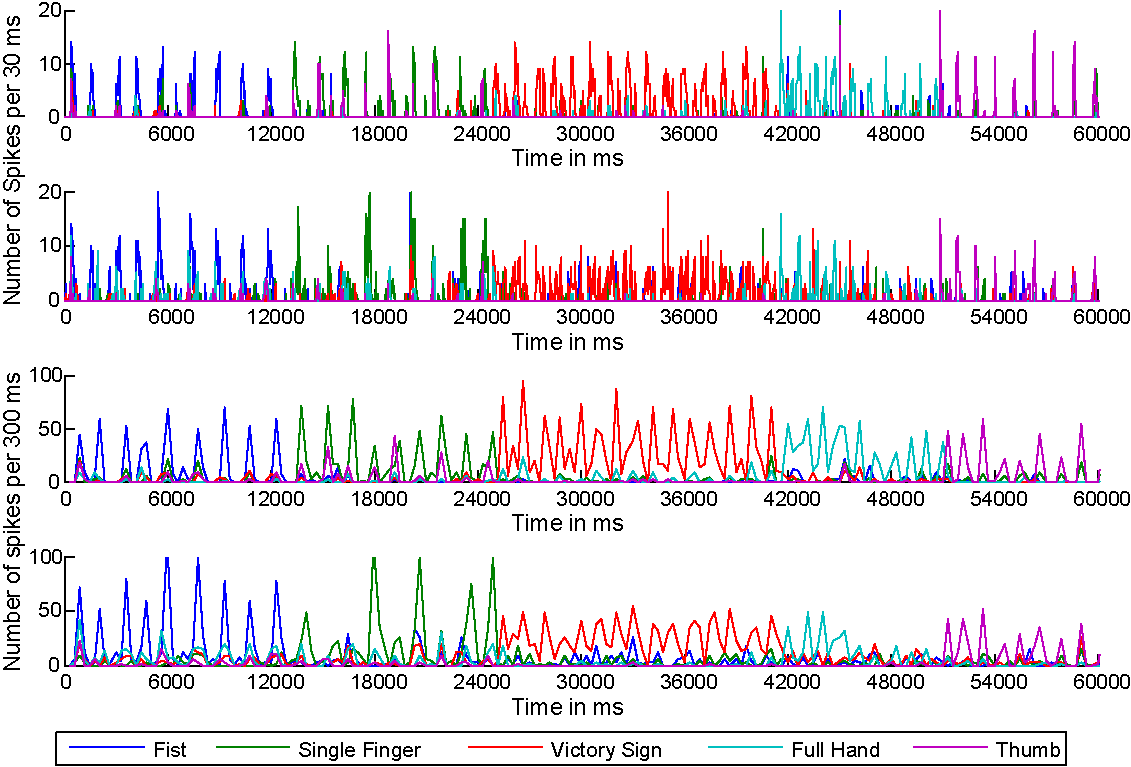
\includegraphics[width=0.48\textwidth]{pics/rateSpiNN.pdf}
	\caption{Real-time neural responses of two experiments on SpiNNaker with time to the same recorded postures.
	These two experiments only differ in input resolution.
	The result of the high input resolution test is plotted the first with a sample frame of 30~ms; 
	while the 3rd plot shows the same result with a sample frame of 300~ms.
	The other two plots refer to the smaller input resolution.
	Every point represents the over all number of spikes of a specific population (different colour) in a `frame'.
	}
	\label{fig:spikerec}
\end{figure}

Correspondingly, the spiking rates of each recognition population is sampled into frames (Figure~\ref{fig:spikerec}) to make a comparison with the Matlab simulation. 
Each colour represents one recognition population, and the spike activity goes higher when the input posture matches the template. 
Firstly, the spike rates are sampled into 30~ms frames which is in accordance with the Matlab experiments.
In the Matlab simulation, the templates are trained with cut frames and so the test images are also fixed to the same length frames.
Otherwise, the recogniser will not work properly because of the replications of the moving posture.
Contrasting this, the spiking rates can be sampled to various frame lengths.
Thus, the other two plots in the figure illustrate the classification in a wider window of 300~ms.
From Table~\ref{tbl:srr}, the recognition and rejection rates are quantified as percentages.

Comparing with the results of Matlab simulation (Table~\ref{tbl:rsl}), the recognition rate is about 7.6\% lower at both high and low resolutions, and the rejection rate remains the same slightly above 75\%. 
However, by changing the frame length to 300~ms recognition rates reach (93.0\% for the larger network) or exceed (86.4\% for smaller network ) the Matlab simulation, meanwhile the rejection rates also drop dramatically by 26.0\% and 22.4\%.
This is in accordance with natural visual responses, which means, the longer an object shows, the more accurate the recognition will be.
Between the two network scales there is also a smaller gap in recognition rates as the window length grows, i.e. 8.9\% and 6.6\% respectively.
%Considering the cost and performance trade-off, with only 1/10th resources required, the small network, is acceptable and can be even improved after applying tracking and learning.
%Regarding the latency between the retinal input and the recognition, we compared the spiking peak of the Matlab simulation and the real-time SpiNNaker test.
%The overall latency is about 1150~ms from a posture being shown to its recognition. 

\begin{figure}
\centering
	\begin{subfigure}[t]{0.24\textwidth}
		\includegraphics[width=\textwidth]{pics/figure_r.png}
	    \caption{Retinal input population }
	    \label{fig:ssa}
	\end{subfigure}
	\begin{subfigure}[t]{0.24\textwidth}
		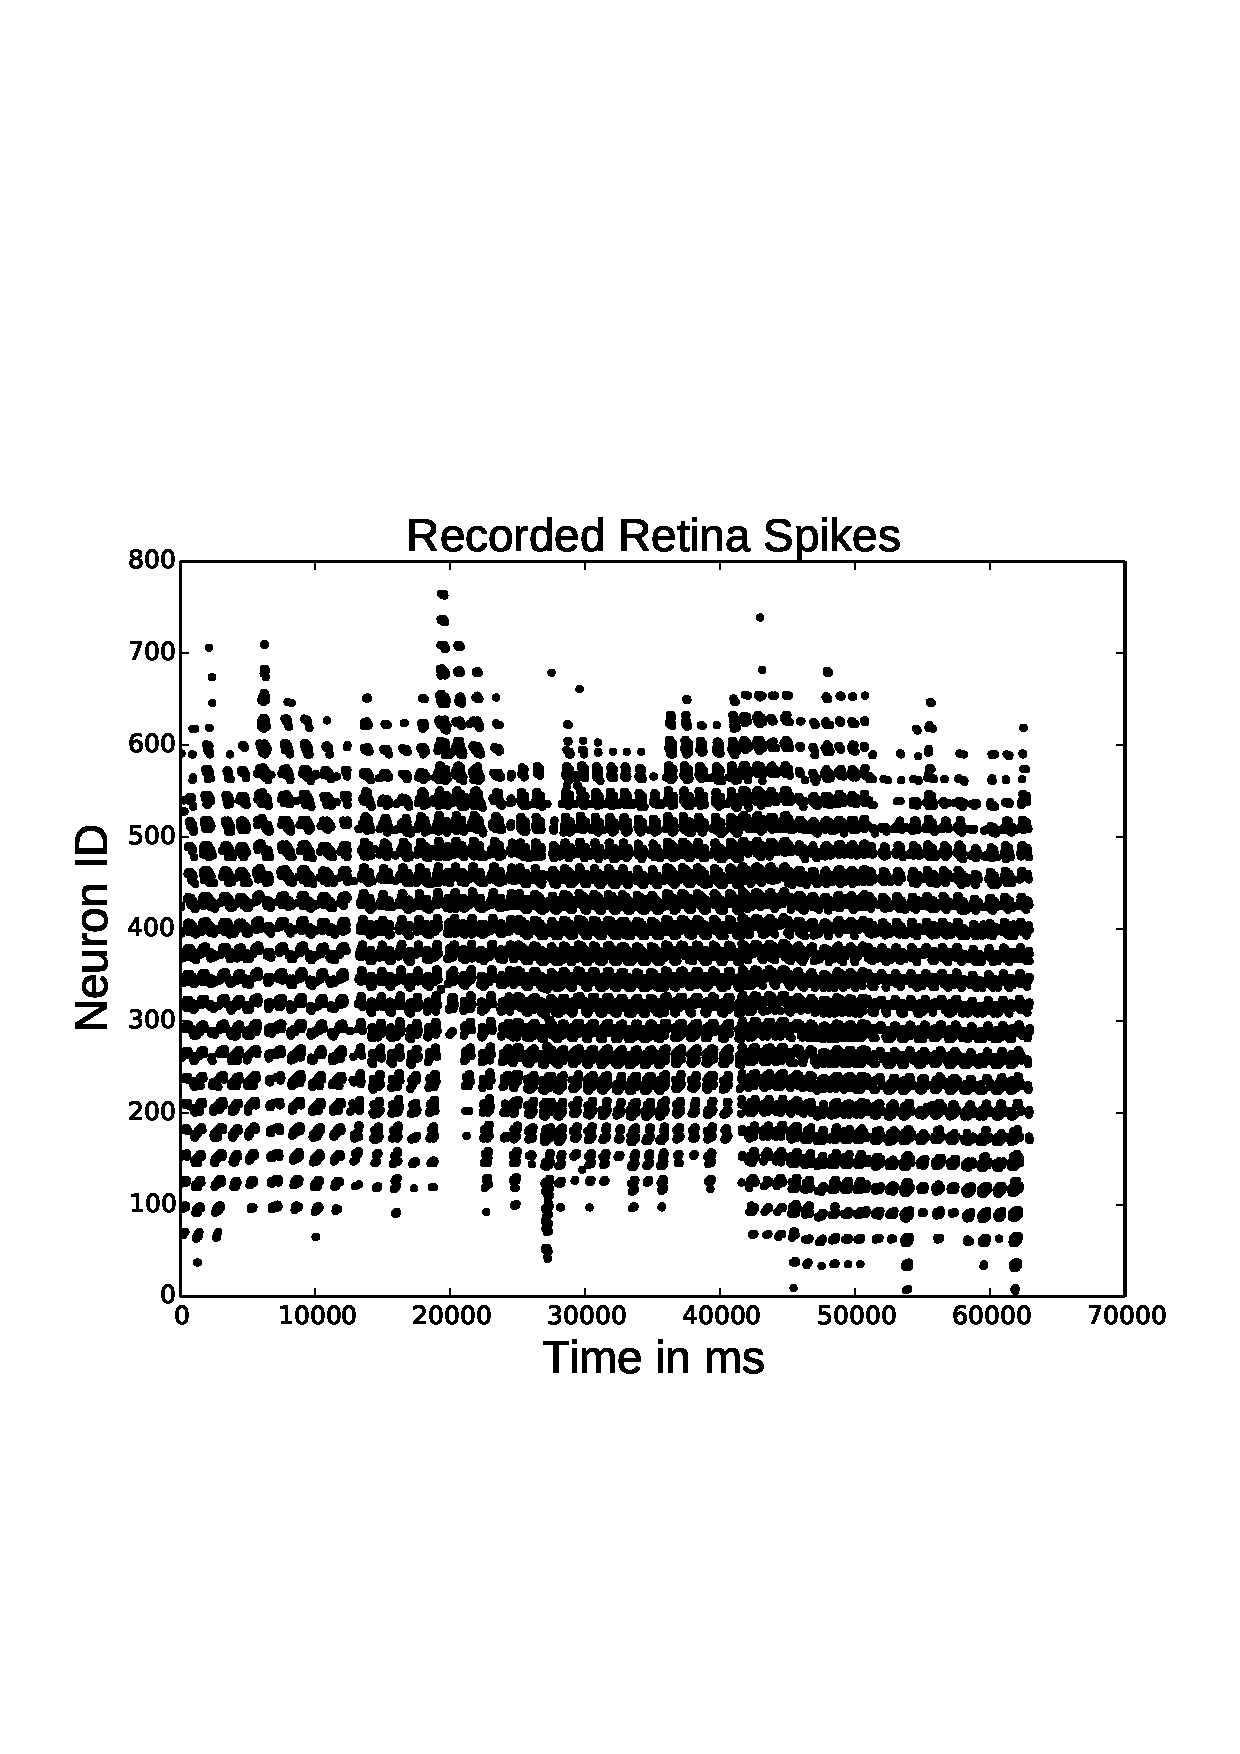
\includegraphics[width=\textwidth]{pics/figure_1.png}
		\caption{Template matching population, `Fist'}
	    \label{fig:rec0}
	\end{subfigure}
	\\
	\begin{subfigure}[t]{0.24\textwidth}
		\includegraphics[width=\textwidth]{pics/figure_2.png}
		\caption{Template matching population, `Index Finger'}
	    \label{fig:rec1}
	\end{subfigure}	
	\begin{subfigure}[t]{0.24\textwidth}
		\includegraphics[width=\textwidth]{pics/figure_3.png}
		\caption{Template matching population, `Victory Sign'}
	\end{subfigure}	
	\\
	\begin{subfigure}[t]{0.24\textwidth}
		\includegraphics[width=\textwidth]{pics/figure_4.png}
		\caption{Template matching population, `Full Hand'}
	    \label{fig:rec5}
	\end{subfigure}	
	\begin{subfigure}[t]{0.24\textwidth}
		\includegraphics[width=\textwidth]{pics/figure_5.png}
		\caption{Template matching population, `Thumb Up'}
	    \label{fig:rect}
	\end{subfigure}	
\caption{Spikes captured during the live recognition of the recorded retinal input with the resolution of 128$\times$128. }
\label{fig:rps}
\end{figure}
\begin{figure}
\centering
	\begin{subfigure}[t]{0.24\textwidth}
		\includegraphics[width=\textwidth]{pics/figure_32_r.png}
	    \caption{Retinal input population }
	    \label{fig:ssa32}
	\end{subfigure}
	\begin{subfigure}[t]{0.24\textwidth}
		\includegraphics[width=\textwidth]{pics/figure_32_1.png}
		\caption{Template matching population, `Fist'}
	    \label{fig:rec032}
	\end{subfigure}
	\\
	\begin{subfigure}[t]{0.24\textwidth}
		\includegraphics[width=\textwidth]{pics/figure_32_2.png}
		\caption{Template matching population, `Index Finger'}
	    \label{fig:rec132}
	\end{subfigure}	
	\begin{subfigure}[t]{0.24\textwidth}
		\includegraphics[width=\textwidth]{pics/figure_32_3.png}
		\caption{Template matching population, `Victory Sign'}
	\end{subfigure}	
	\\
	\begin{subfigure}[t]{0.24\textwidth}
		\includegraphics[width=\textwidth]{pics/figure_32_4.png}
		\caption{Template matching population, `Full Hand'}
	    \label{fig:rec532}
	\end{subfigure}	
	\begin{subfigure}[t]{0.24\textwidth}
		\includegraphics[width=\textwidth]{pics/figure_32_5.png}
		\caption{Template matching population, `Thumb Up'}
	    \label{fig:rect32}
	\end{subfigure}	
\caption{Spikes captured during the live recognition of the recorded retinal input with the resolution of 32$\times$32. }
\label{fig:rps32}
\end{figure}
\begin{table}
\centering
\caption{Real-time recognition results on SpiNNaker in \%}
	\begin{tabular}{p{0.075\textwidth}|p{0.05\textwidth}<{\centering}|p{0.055\textwidth}<{\centering}|p{0.055\textwidth}<{\centering}|p{0.055\textwidth}<{\centering}|p{0.055\textwidth}<{\centering}}
		%Line 1
		\Xhline{1.2pt}
		    \multicolumn{2}{c|}{}	& \multicolumn{2}{c|}{\textbf{30~ms per frame}}  
		    & \multicolumn{2}{c}{\textbf{300~ms per frame}}
		    \\ \cline{3-6}
		%Line 2
		\multicolumn{2}{c|}{}	& \tabincell{c}{High \\ Resolution}
			& \tabincell{c}{Low \\ Resolution}
			& \tabincell{c}{High \\ Resolution}
			& \tabincell{c}{Low \\ Resolution}
			\\ \Xhline{1.2pt}
		%Line 3-4	
		\multirow{2}{*}{\tabincell{l}{\textbf{Fist}}}
			& Correct & 91.78	& 78.02	& 100	& 92.31
			\\ \cline{2-6}
			& Reject  & 82.78 & 78.54 	& 70.73	& 68.29
			\\ \hline
		%Line 5-6
		\multirow{2}{*}{\tabincell{l}{\textbf{Index Finger}}}
			& Correct & 78.25	& 78.25	& 88.24	& 72.22
			\\ \cline{2-6}
			& Reject & 80.46	& 73.56 	& 57.50	& 55.00
			\\ \hline
		%Line 7-8
		\multirow{2}{*}{\tabincell{l}{\textbf{Victory Sign} }}
			& Correct & 96.48	& 86.27	& 95.00	& 92.50
			\\ \cline{2-6}
			& Reject & 64.46	& 72.68 	& 28.57	& 28.57
			\\ \hline
		%Line 9-10
		\multirow{2}{*}{\tabincell{l}{\textbf{Full Hand}}}
			& Correct & 85.29	& 60.78	& 90.00	& 75.00
			\\ \cline{2-6}
			& Reject & 67.31	& 83.65 	& 35.48	& 61.29
			\\ \hline
		%Line 10-11
		\multirow{2}{*}{\tabincell{l}{\textbf{Thumb up}}}
			& Correct & 84.09	& 88.10	& 91.67	& 100
			\\ \cline{2-6}
			& Reject & 87.54	& 73.81 	& 66.67	& 66.67
			\\ \hline\hline
		\multirow{2}{*}{\tabincell{l}{\textbf{Average}}}
			& Correct & 87.18	& 78.28	& 92.98	& 86.41
			\\ \cline{2-6}
			& Reject & 76.51	& 76.45 	& 51.79	& 55.96
			\\ \hline
	\end{tabular}
	\label{tbl:srr}
\end{table}

\section{Conclusion and Future Work}
\label{sec:cfw}

%Motivation
To explore how brain may recognise objects in its general, accurate and energy-efficient manner, this paper proposes the use of a neuromorphic hardware system which includes a DVS retina connected to SpiNNaker, a real-time SNN simulator.
%Problem
Building a recognition system based on this bespoke hardware for dynamic hand postures is a first step in the study of visual pathway of the brain.
%Methods
Inspired by the structures of the primary visual cortex, convolutional neural networks are modelled using both linear perceptrons and LIF neurons.
%Results
The larger network of 74,210 neurons and 15,216,512 synapses runs smoothly in real-time on SpiNNaker using 290 cores within a 48-node board.
The smaller network using 1/10 of the resources is able to recognise the postures in real-time with an accuracy about 86.4\% in average, which is 
only 6.6\% lower than the former but with a better cost/performance ratio.
%In this paper, we implement a dynamic hand posture recognition system running completely on a hardware neuromorphic platform.
%The SNN based classifier is able to recognise moving hand postures instead of static digit or face recognition proposed before.
%The network model is translated from linear perceptrons to LIF spiking neurons with a 10\% drop of accuracy in 30~ms windowing;
%while the performance reaches and even exceeds the perceptrons version when the window length is set to 300~ms.
%Various network sizes are configured to explore the cost and performance trade-off.
%In the tests of linear perceptrons the recognition rate of the smaller network is \% lower for the template matching model and \% lower for the trained MLP model.
%For the SNN based real-time experiments, both the larger network with $74,320$ LIF neurons and $15,216,512$ synapses, and the smaller network with 1/10 of the neurons and 1/50 of the synapses run smoothly on SpiNNaker.
%The gap of recognition rate narrows when the spiking rate is sampled into wider frame of 300~ms.
%The recognition rates of both linear perceptrons (\%) and spiking neurons (\%) with 32 $\times$ 32 input resolution are adequate for the recognition of the moving hand postures.
%This work is a good attempt to start exploring the visual process of the brain.

%Later, we will look more into the overall network latency, which could be due to the system latency and the performance of the rate coding.  
The future work on this topic will include further collaboration with biologists and neuroscientists working on vision systems, especially concentrating on the orientation detection region of the brain.
To equip the system with tracking is another importance direction for future development where the recognition performance can be increased by exploiting short-term memory of a gesture's route.
Using the approch of HMMs~\cite{elmezain2009hidden} and applying to spiking neural networks is an idea we wish to explore as part of this promising work.
%Using the idea of HMMs~\cite{elmezain2009hidden} to spiking neural networks may be a good approach. 
\section{Acknowledgement}
\label{sec:ack}
This research was supported by Samsung under their GRO programme.
The authors appreciate the collaboration with Prof. Bernab{\'e} Linares-Barranco and Luis Camunas-Mesa on the silicon retina.
The authors would also like to thank the meaningful discussions with Evangelos Stromatias, Patrick Camilleri and Michael Hopkins.
Finally, thanks to Jonathan Heathcote and Cameron Patterson for their final proofreading of the paper.
\bibliography{refs}    % this causes the references to be listed
\bibliographystyle{ieeetr}

%\begin{biography}[{\includegraphics[width=1in,height=1.25in,clip,keepaspectratio]{mshell}}]{Michael Shell}
%\end{biography}
\begin{IEEEbiography}[{\includegraphics[width=1in,height=1.25in,clip,keepaspectratio]{pics/liuq.jpg}}]{Qian Liu}
received the B.Sc. degree in
software engineering from Beijing University of Technology, Beijing, China, in 2008.
She started the Ph.D. Study in The University of Manchester in 2014 working on visual and auditory processing with spiking neurons on neuromorphic system.
\end{IEEEbiography}
\begin{biography}[{\includegraphics[width=1in,height=1.25in,clip,keepaspectratio]{pics/sf.jpg}}]{Steve Furber}

(Fellow, IEEE) was born in Manchester, U.K., in 1953. 
He received the B.A.degree in mathematics and the Ph.D. degree in aerodynamics from the University of Cambridge, Cambridge, U.K., in 1974 and 1980, respectively, and honorary doctorates from Edinburgh University, Edinburgh, U.K., in 2010 and Anglia Ruskin University, Cambridge, U.K., in 2012.

From 1978 to 1981, he was Rolls Royce Research Fellow in Aerodynamics at Emmanuel College, Cambridge, U.K., and from 1981 to 1990, he was at Acorn Computers Ltd., Cambridge, U.K., where he was a principal architect of the BBC Microcomputer, which introduced computing into most U.K. schools, and the ARM 32-bit RISC microprocessor, over 40 billion of which have been shipped by ARM Ltd.’s partners.
In 1990, he moved to the ICL Chair in Computer Engineering at the University of Manchester, Manchester, U.K., where his research interests include asynchronous
digital design, low-power systems on chip, and neural systems engineering.

Prof. Furber is a Fellow of the Royal Society, the Royal Academy of Engineering, the British Computer Society, the Institution of Engineering and Technology and the Computer History Museum (Mountain View, CA).
He was a Millennium Technology Prize Laureate (2010) and holds an IEEE Computer Society Computer Pioneer Award (2013).
\end{biography}
\end{document}
